\documentclass[11pt,a4paper]{article}
\usepackage[a4paper,margin=2.3cm]{geometry}
\usepackage{amsmath,amssymb,mathtools}
\usepackage{fontspec}
\usepackage{polyglossia}
\setmainlanguage{english}
\setotherlanguage{russian}
\setmainfont{Liberation Serif}
\setsansfont{Liberation Sans}
\setmonofont{Liberation Mono}
\newfontfamily\cyrillicfont[Ligatures=TeX]{Liberation Serif}
\newfontfamily\cyrillicfontsf[Ligatures=TeX]{Liberation Sans}
\newfontfamily\cyrillicfonttt{Liberation Mono}
\usepackage{booktabs}
\usepackage{array}
\usepackage{enumitem}
\usepackage{graphicx}
\usepackage{float}
\usepackage{xcolor}
\usepackage[hidelinks]{hyperref}

\setlength{\parindent}{0pt}
\setlength{\parskip}{0.55em}
\emergencystretch=1.5em
\setlist{itemsep=0.25em,topsep=0.3em}

\newcommand{\norm}[1]{\lVert #1\rVert_2}
\newcommand{\E}{\mathbb{E}}
\DeclareMathOperator{\diag}{diag}
\DeclareMathOperator{\sigm}{sigm}
\DeclareMathOperator{\Var}{Var}
\makeatletter\newcommand{\tabinput}[1]{\@@input #1 }\makeatother

\title{Section 3: Required simulations\\[0.2em]
\large logistic regression and a two-layer network, SGD versus R-SGD}
\author{Homework Mini-Project: SGD versus Robust SGD under Gradient Uncertainty}
\date{17 November 2026}

\begin{document}
\maketitle

\section*{Statement and summary}

Section 3 asks for two simulations: single-layer logistic regression on Gaussian
blobs and a two-layer $\tanh$ network on noisy semicircles. In each, SGD and R-SGD are
compared under gradient uncertainty, with clean evaluation and at least one noise-free and
one noisy level. For each simulation the following are required: training and validation
loss curves at all noise levels, the final training loss, test loss, accuracy, runtime and
zero-step frequency, a decision boundary for a stated evaluation seed, and a discussion of
whether optimisation and prediction give the same ranking. A fair comparison also needs the
tuning and evaluation protocol of Section 4, so its parts 1--4 are implemented here as well.

Main findings. They are empirical findings for these two problems and these settings, not
general statements.
\begin{itemize}
\item \textbf{Logistic regression.} Both methods reach the Bayes accuracy
($0.922$ vs.\ the Bayes rule's $0.923$ on the same test sets) at every noise level except the
largest. R-SGD lowers the training loss slightly at $c=0,1$ (by $0.001$--$0.003$, consistent
within a fixed data set: 10/10 and 9/10 seeds), but accuracy does not change. With the settings
frozen at $c=1$, R-SGD is worse than SGD at $c=4$ and clearly worse at $c=16$.
\item \textbf{Two-layer network.} Without artificial noise, R-SGD reaches a much lower
training loss ($0.0019$ vs.\ $0.0110$, 10/10 seeds) and lower test loss (9/10), but not a
higher accuracy (3 wins, 2 ties). An SGD run with the same mean step length is as good
(R-SGD wins 4/10). For $c\ge1$ the frozen R-SGD setting is worse than SGD on test loss and
accuracy, and at $c=16$ it fails in 8 of 10 seeds (final loss above the initial
$\log 2$).
\item \textbf{Why.} When the injected noise dominates, $S_k\approx sI$ and the robust step
reduces to SGD with the step size multiplied by about $(1-\rho/\sqrt p)$. The measured step
ratios are $0.744$, $0.505$, $0.269$ for $\rho/\sqrt p=0.25,0.5,0.75$. Such a step does not
remove noise; it only shortens the step, and it shrinks large (noisy) gradients relatively
\emph{less}. Where R-SGD improved the loss in the radius sweep, a step-length-matched SGD
did the same or better, with one exception: at low noise in logistic regression, R-SGD's
SNR-dependent shrinkage beat a constant step reduction on loss (5/5 seeds at every radius), as an
adaptive schedule, but again without changing accuracy.
\item \textbf{Zero steps before a minimiser.} For the network, radii
$\rho\gtrsim\sqrt p$ produce 35--100\% zero steps and stop training far from any minimiser
(test accuracy $0.86$--$0.50$); with noise and $\rho=2\sqrt p$ the network never leaves its
initialisation.
\item \textbf{Optimisation vs.\ prediction.} At low noise the ranking by training loss agrees
with the ranking by test loss but not with accuracy (agreement $2$--$5$ of 10 seeds). At high
noise all three rankings agree (SGD better).
\end{itemize}

\section*{Step 1. Common protocol}

\begin{center}
\small
\begin{tabular}{@{}p{0.27\linewidth}p{0.68\linewidth}@{}}
\toprule
Item & Choice and reason \\
\midrule
Data & balanced classes; $n_{\rm train}=400$, $n_{\rm val}=400$, $n_{\rm test}=4000$ drawn
independently (large test set: the standard error of accuracy is $\le0.005$) \\
Preprocessing & standardisation $a\mapsto(a-\bar a_{\rm train})/s_{\rm train}$ with the
\emph{training} mean and standard deviation only, applied to all three sets \\
Loss & $\ell(t,y)=\log(1+e^t)-yt$, evaluated as \texttt{logaddexp(0,t)-y*t}; objective = mean
training loss, no regulariser; class $=\mathbf 1[t>0]$ \\
Batch and budget & $b=16$, sampling with replacement; $K=500$ updates (logistic), $K=3000$
(network); $bK$ gradient evaluations per run for both methods \\
Step sizes & $\alpha_k=\alpha_0/\sqrt{1+k/50}$ for both methods \\
Gradient noise & $v_{k,i}=u_i(\theta_k)+\sigma z_{k,i}$, $z_{k,i}\sim\mathcal N(0,I_p)$, i.i.d.\
across observations and iterations; $\sigma=c\,\gamma$, $c\in\{0,1,4,16\}$ \\
Noise unit $\gamma$ & RMS of the clean per-example gradients at the initial point, averaged
over the tuning seeds: $\gamma=0.500$ (logistic), $\gamma=0.215$ (network) \\
Uncertainty model & $g_k$, $S_k$ from formula (4) applied to the \emph{same} $b$ observations
used in the update \\
Evaluation & every loss and accuracy on clean data; 61 checkpoints per run for the curves \\
\bottomrule
\end{tabular}
\end{center}

\textbf{Noise levels.} $c=0$ is the case without artificial perturbation (mini-batch sampling
noise only). With $c=1$ the perturbation of one observation is as large as a typical
per-example gradient coordinate. With $c=4$ and $c=16$ it dominates. After averaging over
$b=16$ observations, the injected noise in $g_k$ has standard deviation $c\gamma/4$ per
coordinate.

\textbf{Radius scale.} The radius is parametrised as $\rho=r\sqrt p$. Near a stationary
point $g_k^TS_k^{-1}g_k$ is approximately $\chi^2_p$ with mean $p(b-1)/(b-3)$ (Section 2,
step 5), so the threshold of the zero-step rule scales with $\sqrt p$. A fixed $\rho$ would mean
very different things for $p=3$ and $p=33$; with $r$ the meaning is the same: $r\approx1$ is
the point where zero steps begin near a minimiser.

\textbf{Tuning (Section 4.2).}
\begin{itemize}
\item Grids: $\alpha_0\in\{0.1,0.3,1,3,10,30\}$ for both methods; $r\in\{0,0.25,0.5,0.75,1,1.25\}$
for R-SGD. $r=0$ is included, and R-SGD with $r=0$ is SGD.
\item Tuning data: 3 tuning seeds with their own data sets, initialisations, batches and noise,
disjoint from all evaluation seeds; tuning noise level $c=1$. Test data are never used.
\item Criterion: mean over tuning seeds of the validation loss averaged over the last 5 of 61
checkpoints. A run is marked failed if its training loss becomes non-finite or exceeds 50 times
its initial value.
\item Search budgets: SGD $6\times3=18$ runs, R-SGD $36\times3=108$ runs. The larger R-SGD
budget favours R-SGD (it is the minimum over more noisy estimates); this is discussed below.
\item Settings are frozen after tuning and then used unchanged at every noise level.
\end{itemize}

\textbf{Evaluation (Section 4.3).} Two designs, each with 10 seeds, paired across methods
(same data, initialisation, batch indices and noise draws $z_{k,i}$):
\begin{itemize}
\item \textbf{A} (data set varies): every seed draws a new training, validation and test set,
a new initialisation, new batches and new noise. Spread in A combines uncertainty across data
sets and training randomness.
\item \textbf{B} (training randomness only): the data set of A-seed 0 is fixed; initialisation,
batches and noise vary.
\end{itemize}
Error bars: ``mean $\pm$ sd'' is the mean and the sample standard deviation over the 10 seeds
(the spread of outcomes). For paired differences ``mean $\pm$ h'' gives the half-width $h$ of
the 95\% $t$-interval for the mean difference, and ``wins'' counts seeds where R-SGD is better
(ties in parentheses).

\textbf{Extras (Section 4.4).} (i) A radius sweep $r\in\{0,\dots,2\}$ at SGD's tuned $\alpha_0$,
5 seeds. (ii) A step-length-matched SGD control: SGD with
$\alpha_0'=\alpha_0\cdot\overline{\|d_k\|/(\alpha_k\|g_k\|)}$, the mean step ratio of the
corresponding R-SGD runs (zero steps count as 0). It is run for the frozen setting and for every
point of the sweep, on the same seeds.

\section*{Step 2. Simulation 1: logistic regression}

\subsection*{2.1 Model, gradient and reference}

$a\mid y\sim\mathcal N\big((2y-1)(1,1)^T,I_2\big)$, $t_\theta(a)=w^Ta+c$, $\theta=(w_1,w_2,c)$,
$p=3$, $\theta_0=0$ (the problem is convex, so a fixed start is natural). The per-example
gradient is $u_i(\theta)=(\sigm(t_i)-y_i)\,(a_i^T,1)^T$ (Section 2, step 3). The
finite-difference check at the evaluation data gives relative errors $2.7\cdot10^{-10}$ (mean
gradient) and $1.9\cdot10^{-10}$ (per example).

\textbf{Reference.} The model is well specified: the log-likelihood ratio is
$\log\frac{p(a\mid1)}{p(a\mid0)}=2\,(1,1)a$, so the Bayes rule is $a_1+a_2>0$, with accuracy
$\Phi(\sqrt2)\approx0.921$. On the actual test sets of design A the Bayes rule has accuracy
$0.9228\pm0.0031$ and test loss $0.1905\pm0.0065$ (true logit $2(a_1+a_2)$). No method
can do better on average.

\subsection*{2.2 Tuning}

\begin{figure}[H]
\centering
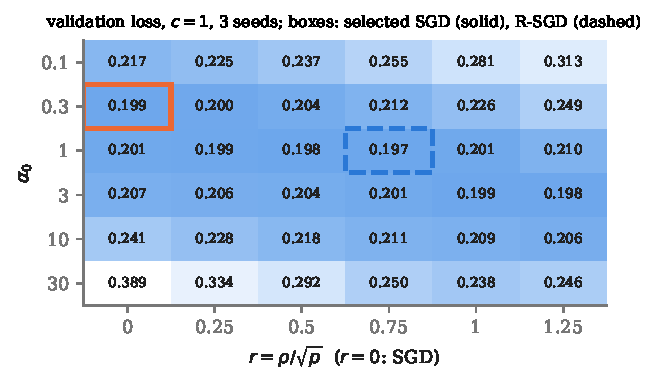
\includegraphics[width=0.49\linewidth]{../fig3/logreg_tuning.pdf}\hfill
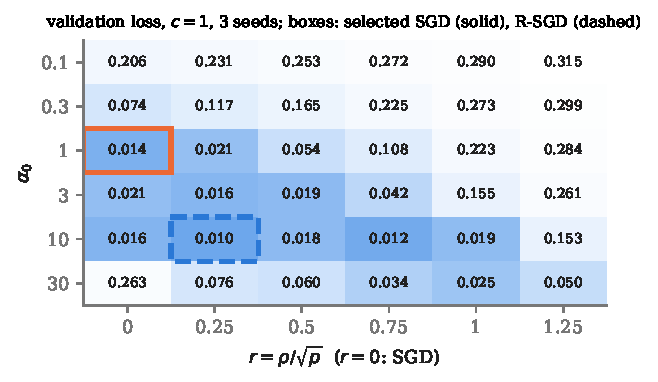
\includegraphics[width=0.49\linewidth]{../fig3/mlp_tuning.pdf}
\caption{Tuning criterion (mean validation loss, $c=1$, 3 tuning seeds) for logistic regression
(left) and the network (right). Column $r=0$ is SGD. Boxes mark the selected settings.}
\label{fig:tuning}
\end{figure}

Selected: SGD $\alpha_0=0.3$; R-SGD $\alpha_0=1$, $r=0.75$ ($\rho=1.30$). Neither lies on the
edge of the grid. The criterion is very flat: 10 of 36 cells are within $0.005$ of the best
($0.197$). The low region runs along a diagonal: a larger $\alpha_0$ is compensated by a larger
$r$, e.g.\ $(1,0.75)$, $(3,1)$, $(3,1.25)$ are almost equal. This is the trade-off between
learning rate and radius asked about in Section 5(b): both control the effective step length.

\subsection*{2.3 Results}

\begin{figure}[H]
\centering
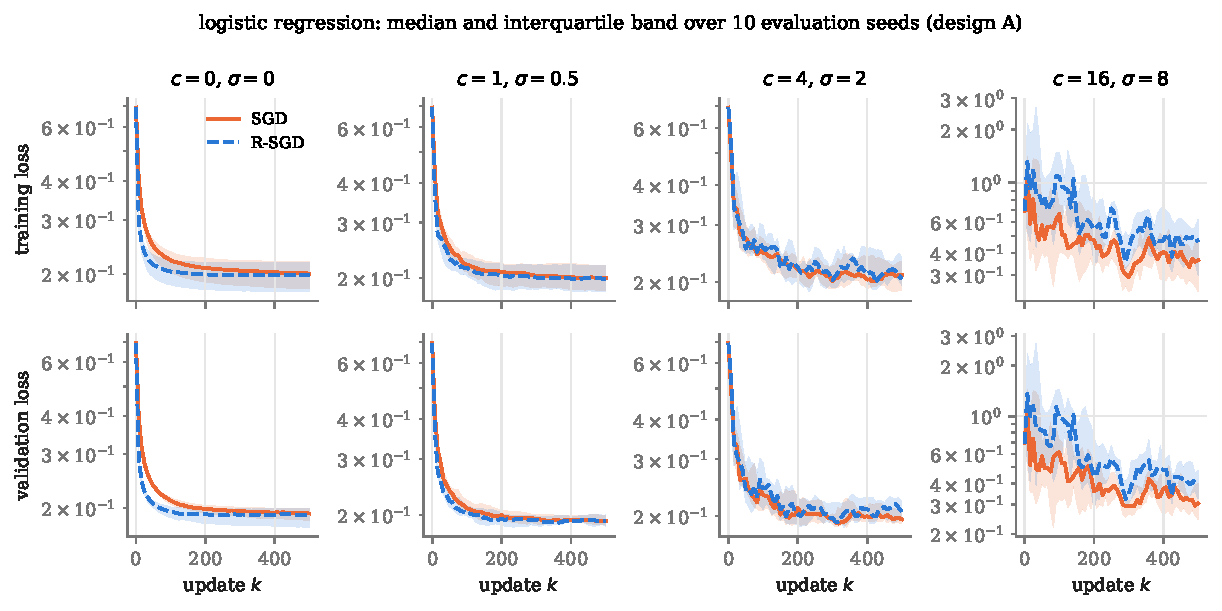
\includegraphics[width=\linewidth]{../fig3/logreg_curves.pdf}
\caption{Logistic regression: training (top) and validation (bottom) loss on clean data
against updates, median and interquartile band over 10 evaluation seeds (design A). Frozen
settings: SGD $\alpha_0=0.3$; R-SGD $\alpha_0=1$, $\rho=1.30$.}
\label{fig:lr_curves}
\end{figure}

\begin{center}
\small
\setlength{\tabcolsep}{4pt}
\begin{tabular}{@{}clccccc@{}}
\toprule
$c$ & method & final train loss & test loss & test accuracy & zero steps & time, ms (µs/update) \\
\midrule
\tabinput{../tabs3/tab_lr_main.tex}
\bottomrule
\end{tabular}

\smallskip
Logistic regression, design A, mean $\pm$ sd over 10 seeds; $bK=8000$ gradient evaluations per
run for both methods; Bayes rule: accuracy $0.9228$, test loss $0.1905$.
\end{center}

\begin{center}
\small
\setlength{\tabcolsep}{2.6pt}
\begin{tabular}{@{}cccccccccc@{}}
\toprule
& & \multicolumn{2}{c}{$\Delta$ train loss} & \multicolumn{2}{c}{$\Delta$ test loss}
& \multicolumn{2}{c}{$\Delta$ accuracy} & \multicolumn{2}{c}{ranking agreement} \\
\cmidrule(lr){3-4}\cmidrule(lr){5-6}\cmidrule(lr){7-8}\cmidrule(lr){9-10}
$c$ & design & mean $\pm$ h & wins & mean $\pm$ h & wins & mean $\pm$ h & wins (ties) & tr$\to$te & tr$\to$acc \\
\midrule
\tabinput{../tabs3/tab_lr_paired.tex}
\bottomrule
\end{tabular}

\smallskip
Paired differences R-SGD $-$ SGD (negative loss and positive accuracy differences favour
R-SGD); ``ranking agreement'': number of seeds in which the sign of $\Delta$ train loss
predicts the sign of $\Delta$ test loss (tr$\to$te) or of $-\Delta$ accuracy (tr$\to$acc).
\end{center}

Reading.
\begin{itemize}
\item \textbf{Accuracy is saturated.} At $c\le4$ both methods are within $0.005$ of the Bayes
accuracy, and the mean accuracy difference is below $0.001$ in absolute value. Loss differences
of a few thousandths move the linear boundary by a negligible amount
(Figure~\ref{fig:lr_bound}).
\item \textbf{Small, consistent loss gain at $c\le1$.} Within a fixed data set (design B) R-SGD
has a lower training loss in 10/10 ($c=0$) and 9/10 ($c=1$) seeds and lower test loss in 10/10
and 8/10. Across data sets (design A) the same differences are hidden by the much larger
data-set spread (sd of test loss $0.007$ in A vs.\ $0.001$ in B at $c=0$).
\item \textbf{Worse at $c\ge4$ with frozen settings.} R-SGD runs with $\alpha_0=1$, three times
SGD's step size, and relies on shrinkage to compensate. When noise dominates, the shrinkage is
nearly a constant factor (step 4), large noisy gradients pass through, and the loss is higher:
$+0.005$ at $c=4$ and $+0.095$ at $c=16$, SGD better in 7--8 of 10 seeds.
\item \textbf{Zero steps:} 18\% of updates at $c=0$ and 32--33\% at $c\ge1$, including
updates early in training. They did not prevent convergence because $p=3$ and the remaining steps
are large.
\item \textbf{Runtime:} SGD 16--21\,µs per update, R-SGD 58--88\,µs (2.8--4.4 times more),
with identical gradient-evaluation counts.
\end{itemize}

\begin{figure}[H]
\centering
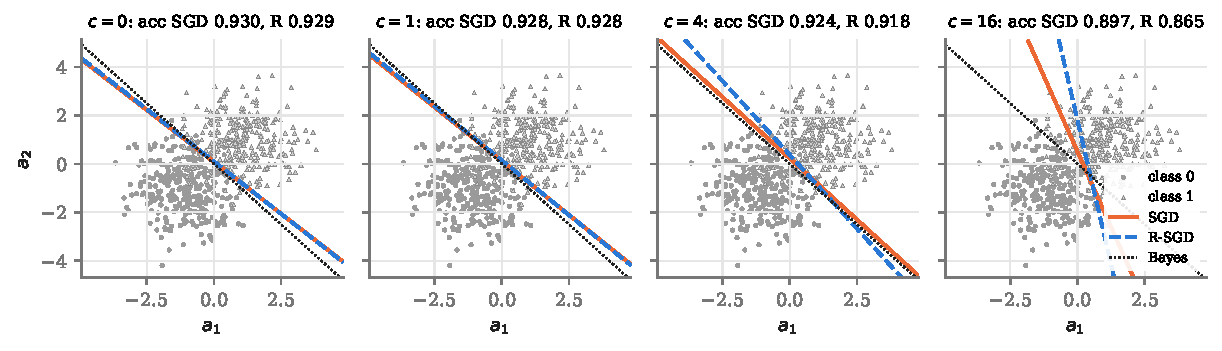
\includegraphics[width=\linewidth]{../fig3/logreg_boundaries.pdf}
\caption{Logistic regression, evaluation seed A-0 (data seed listed in step 6): decision
boundaries $t_\theta(a)=0$ of the final SGD and R-SGD iterates in original coordinates, the
Bayes boundary $a_1+a_2=0$, and 600 test points.}
\label{fig:lr_bound}
\end{figure}

\subsection*{2.4 Step length, sensitivity and variability}

\begin{center}
\small
\setlength{\tabcolsep}{4pt}
\begin{tabular}{@{}cccccccc@{}}
\toprule
$c$ & step ratio & $\alpha_0'$ & R-SGD test loss & matched SGD test loss & $\Delta$ (R $-$ matched) & wins & acc R / matched \\
\midrule
\tabinput{../tabs3/tab_lr_matched.tex}
\bottomrule
\end{tabular}

\smallskip
Frozen R-SGD versus SGD with the same mean step length, design A, 10 seeds.
\end{center}

At $c=0$ the matched step size is exactly SGD's tuned $0.3$, and the two methods tie (5/10).
At $c=1$, R-SGD beats the matched SGD in 9/10 seeds by $0.003$ in test loss. At $c\ge4$ the
matched SGD is better, at $c=16$ by $0.14$.

\begin{figure}[H]
\centering
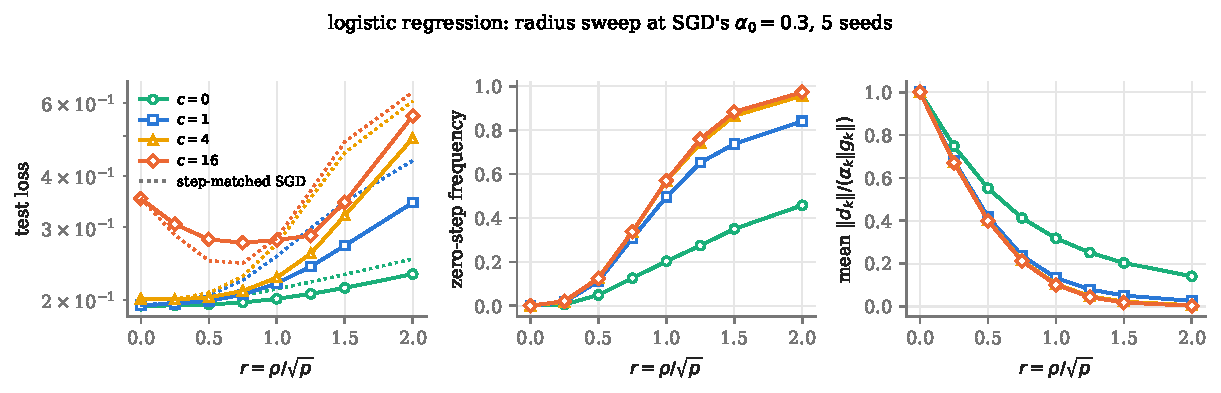
\includegraphics[width=\linewidth]{../fig3/logreg_sensitivity.pdf}
\caption{Logistic regression, radius sweep at SGD's $\alpha_0=0.3$, 5 seeds. Left: test loss of
R-SGD (solid) and of step-length-matched SGD (dotted). Middle: zero-step frequency. Right: mean
step ratio $\|d_k\|/(\alpha_k\|g_k\|)$.}
\label{fig:lr_sens}
\end{figure}

\begin{center}
\small
\setlength{\tabcolsep}{4pt}
\begin{tabular}{@{}ccccccccc@{}}
\toprule
$c$ & $r$ & zero steps & step ratio & train loss & test loss & matched SGD test & R wins & test acc \\
\midrule
\tabinput{../tabs3/tab_lr_sens.tex}
\bottomrule
\end{tabular}

\smallskip
Logistic regression, radius sweep at $\alpha_0=0.3$ (means over 5 seeds); $r=0$ is SGD.
\end{center}

\begin{itemize}
\item At $c\le4$, increasing $r$ does not lower the loss (at most by $0.0007$ for $r=0.25$,
then it rises): with a tuned SGD step there is nothing to gain. But R-SGD is better than SGD
with the same mean step at every $r$, in 5/5 seeds (4/5 once). Its shrinkage is small early (large gradients, high signal-to-noise ratio) and
large late, i.e.\ it acts as an adaptive decay of the step size; a constant reduction loses
speed early.
\item At $c=16$, $r=0.5$--$0.75$ lowers the test loss from $0.352$ to $0.275$, but the matched SGD
does better ($0.246$, R-SGD wins 1/5): the gain is a step-length effect.
\item Accuracy hardly changes with $r$ (within $0.002$ at $c\le4$) until zero steps dominate.
\end{itemize}

\begin{center}
\small
\begin{tabular}{@{}ccccccccc@{}}
\toprule
& \multicolumn{4}{c}{sd of test loss} & \multicolumn{4}{c}{sd of test accuracy} \\
\cmidrule(lr){2-5}\cmidrule(lr){6-9}
$c$ & SGD A & SGD B & R-SGD A & R-SGD B & SGD A & SGD B & R-SGD A & R-SGD B \\
\midrule
\tabinput{../tabs3/tab_lr_var.tex}
\bottomrule
\end{tabular}

\smallskip
Logistic regression: spread across data sets and training randomness (A) versus training
randomness only (B).
\end{center}
At $c\le1$ the spread across data sets dominates (the sd in A is 2--7 times that in B); at
$c\ge4$ the injected noise makes training randomness the main source.

\section*{Step 3. Simulation 2: two-layer network}

\subsection*{3.1 Model, initialisation, gradient}

Semicircles: $t\sim U[0,\pi]$, class 0 at $(\cos t,\sin t)+e$, class 1 at
$(1-\cos t,\tfrac12-\sin t)+e$, $e\sim\mathcal N(0,0.1^2I_2)$. Model
$t_\theta(a)=w_2^T\tanh(W_1a+b_1)+b_2$ with 8 hidden units, $p=33$. Initialisation:
$W_1\sim\mathcal N(0,\tfrac12)$, $b_1=0$, $w_2\sim\mathcal N(0,\tfrac18)$, $b_2=0$ (variance
$1/\text{fan-in}$), drawn from the seed's initialisation stream; SGD and R-SGD start from the
same $\theta_0$. The initial loss is close to $\log2=0.693$. The gradient is computed by
per-example back-propagation (Section 2, step 3); the finite-difference check at the actual
initial point gives relative errors $4.9\cdot10^{-10}$ (mean) and $8.9\cdot10^{-10}$ (per
example).

\subsection*{3.2 Tuning}

Selected (Figure~\ref{fig:tuning}, right): SGD $\alpha_0=1$; R-SGD $\alpha_0=10$, $r=0.25$
($\rho=1.44$). Neither is on the edge. The R-SGD criterion ($0.0104$) is below SGD's
($0.0138$), but the surface is irregular: $(10,0)$, i.e.\ SGD with $\alpha_0=10$, has $0.0156$,
$(10,0.5)$ has $0.0184$, $(10,0.75)$ has $0.0117$. Such non-monotone neighbours indicate that
differences of this size are within the noise of a 3-seed estimate. Step 3.3 shows the
consequence.

\subsection*{3.3 Results}

\begin{figure}[H]
\centering
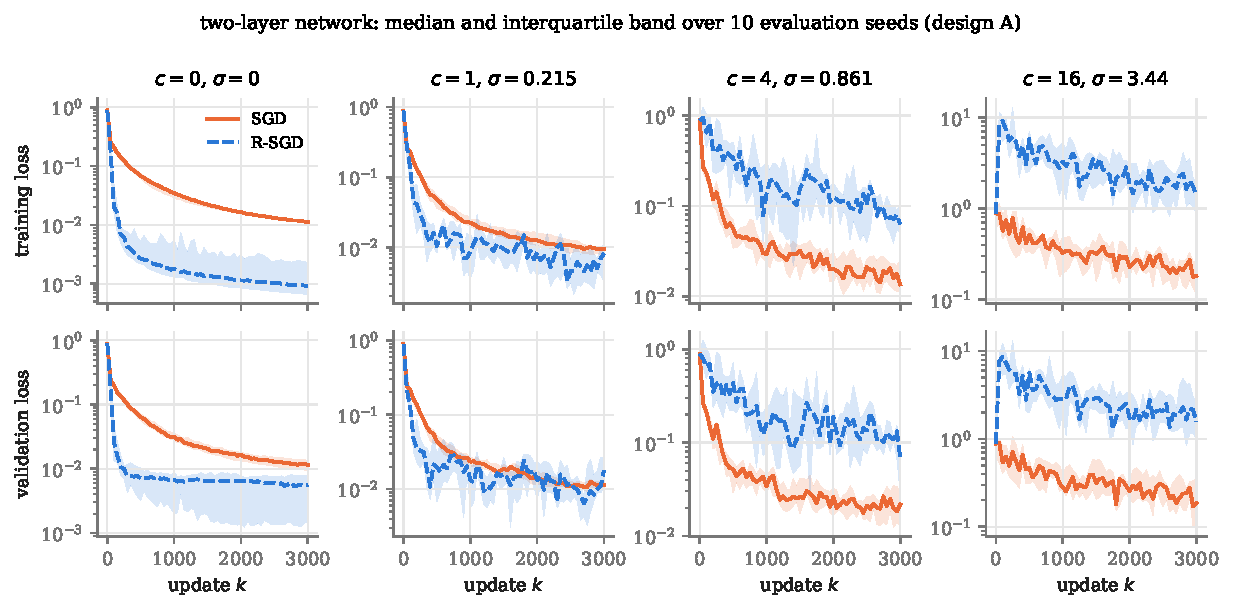
\includegraphics[width=\linewidth]{../fig3/mlp_curves.pdf}
\caption{Two-layer network: training (top) and validation (bottom) loss on clean data, median
and interquartile band over 10 evaluation seeds (design A). Frozen settings: SGD $\alpha_0=1$;
R-SGD $\alpha_0=10$, $\rho=1.44$.}
\label{fig:mlp_curves}
\end{figure}

\begin{center}
\small
\setlength{\tabcolsep}{4pt}
\begin{tabular}{@{}clccccc@{}}
\toprule
$c$ & method & final train loss & test loss & test accuracy & zero steps & time, ms (µs/update) \\
\midrule
\tabinput{../tabs3/tab_mlp_main.tex}
\bottomrule
\end{tabular}

\smallskip
Two-layer network, design A, mean $\pm$ sd over 10 seeds; $bK=48\,000$ gradient evaluations per
run for both methods.
\end{center}

\begin{center}
\small
\setlength{\tabcolsep}{2.6pt}
\begin{tabular}{@{}cccccccccc@{}}
\toprule
& & \multicolumn{2}{c}{$\Delta$ train loss} & \multicolumn{2}{c}{$\Delta$ test loss}
& \multicolumn{2}{c}{$\Delta$ accuracy} & \multicolumn{2}{c}{ranking agreement} \\
\cmidrule(lr){3-4}\cmidrule(lr){5-6}\cmidrule(lr){7-8}\cmidrule(lr){9-10}
$c$ & design & mean $\pm$ h & wins & mean $\pm$ h & wins & mean $\pm$ h & wins (ties) & tr$\to$te & tr$\to$acc \\
\midrule
\tabinput{../tabs3/tab_mlp_paired.tex}
\bottomrule
\end{tabular}

\smallskip
Two-layer network: paired differences R-SGD $-$ SGD, as in the logistic-regression table.
\end{center}

Reading.
\begin{itemize}
\item \textbf{$c=0$: R-SGD optimises faster.} Its training loss is $0.0019$ vs.\ $0.0110$
(10/10 seeds in both designs); test loss is lower in 9/10 (A) and 10/10 (B). The curves in
Figure~\ref{fig:mlp_curves} separate after a few hundred updates. Accuracy is not better (3 wins,
2 ties), because both methods already classify $99.8\%$ of the test points correctly.
\item \textbf{The $c=0$ gain is a step-length gain.} R-SGD's mean step ratio is $0.59$, so it
moves like SGD with $\alpha_0'=5.9$, six times SGD's tuned $1$. That SGD run reaches test loss
$0.0065$ vs.\ R-SGD's $0.0082$ (R-SGD better in 4/10). SGD's $\alpha_0=1$ was chosen at $c=1$
from a noisy criterion, not at $c=0$.
\item \textbf{$c=1$, the tuning level itself: R-SGD is worse.} Its evaluation validation loss is
$0.0230\pm0.0207$ against SGD's $0.0114\pm0.0028$, although tuning had predicted the opposite
($0.0104$ vs.\ $0.0138$). The R-SGD selection was the minimum of 36 noisy estimates against 6 for
SGD, which makes it optimistically biased (the ``winner's curse''), and the chosen large
$\alpha_0=10$ is a high-variance setting. Test accuracy: $0.9946$ vs.\ $0.9980$, SGD better in
8 of 10 seeds (one tie).
\item \textbf{$c\ge4$: the frozen R-SGD setting breaks down.} Test loss $0.115$ vs.\ $0.025$
($c=4$) and $1.96$ vs.\ $0.22$ ($c=16$); at $c=16$, 8 of 10 R-SGD runs end with a training loss
above the initial $\log2$. An effective step size of about $7.4/\sqrt{1+k/50}$, i.e.\ 7.4 times
SGD's, with noise-dominated gradients throws the network into saturated regions. No run met the formal failure criterion (loss $>50$
times the initial loss).
\item \textbf{Zero steps:} none at the selected $\rho=1.44$, which is far below the
noise-dominated threshold $\approx\sqrt{p(b-1)/(b-3)}=6.2$.
\item \textbf{Runtime:} SGD 32--49\,µs per update, R-SGD 109--128\,µs (2.6--3.6 times more).
\end{itemize}

\begin{figure}[H]
\centering
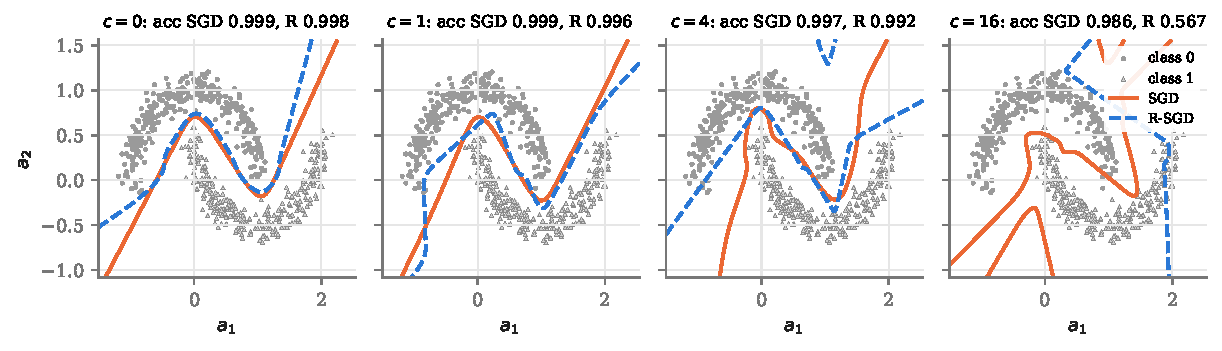
\includegraphics[width=\linewidth]{../fig3/mlp_boundaries.pdf}
\caption{Two-layer network, evaluation seed A-0: decision boundaries of the final SGD and R-SGD
iterates in original coordinates with 600 test points. Away from the data the two boundaries
extrapolate differently even when both separate the semicircles (left two panels).}
\label{fig:mlp_bound}
\end{figure}

\subsection*{3.4 Step length, sensitivity and variability}

\begin{center}
\small
\setlength{\tabcolsep}{4pt}
\begin{tabular}{@{}cccccccc@{}}
\toprule
$c$ & step ratio & $\alpha_0'$ & R-SGD test loss & matched SGD test loss & $\Delta$ (R $-$ matched) & wins & acc R / matched \\
\midrule
\tabinput{../tabs3/tab_mlp_matched.tex}
\bottomrule
\end{tabular}

\smallskip
Two-layer network: frozen R-SGD versus SGD with the same mean step length, design A, 10 seeds.
\end{center}

\begin{figure}[H]
\centering
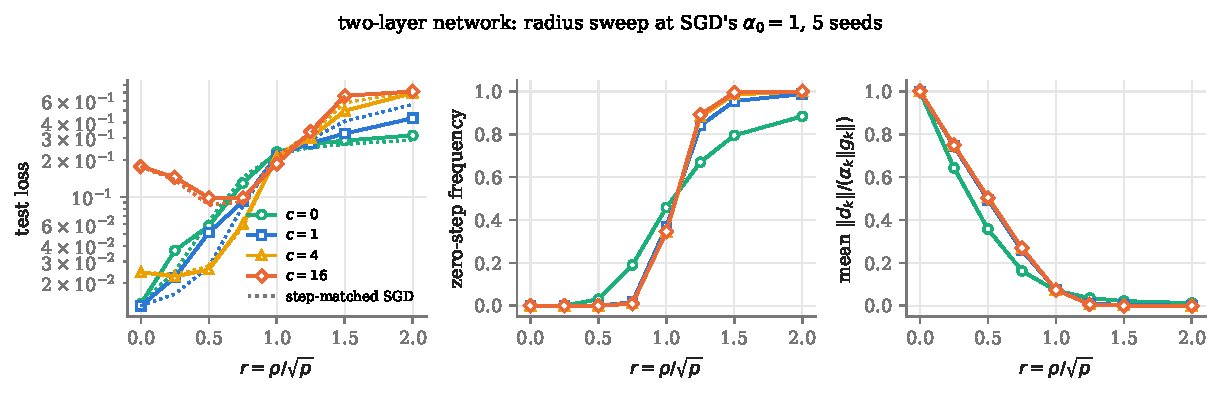
\includegraphics[width=\linewidth]{../fig3/mlp_sensitivity.pdf}
\caption{Two-layer network, radius sweep at SGD's $\alpha_0=1$, 5 seeds. Left: test loss of
R-SGD (solid) and of step-length-matched SGD (dotted). Middle: zero-step frequency. Right: mean
step ratio.}
\label{fig:mlp_sens}
\end{figure}

\begin{center}
\small
\setlength{\tabcolsep}{4pt}
\begin{tabular}{@{}ccccccccc@{}}
\toprule
$c$ & $r$ & zero steps & step ratio & train loss & test loss & matched SGD test & R wins & test acc \\
\midrule
\tabinput{../tabs3/tab_mlp_sens.tex}
\bottomrule
\end{tabular}

\smallskip
Two-layer network, radius sweep at $\alpha_0=1$ (means over 5 seeds); $r=0$ is SGD.
\end{center}

\begin{itemize}
\item At $c\le1$ every $r>0$ worsens the result; at $c=4$ the effect of $r\le0.5$ is within
noise.
\item At $c=16$, $r=0.5$--$0.75$ improves the test loss from $0.176$ to $0.098$ and the
accuracy from $0.953$ to $0.968$, but the matched SGD is better still ($0.086$; R-SGD wins
2/5 and 1/5). In the noise-dominated regime the robust step behaves as a shorter SGD step.
\item \textbf{Zero steps before a minimiser.} For $r\ge1$ the zero-step frequency jumps to
35--100\%, and training stops at test accuracy $0.91$--$0.50$. At $c=4,16$ with $r=2$ the
network practically never moves (99.9--100\% zero steps, accuracy $0.50$). The
explanation (step 4): when noise dominates, $g_k^TS_k^{-1}g_k$ is close to its value at a
stationary point regardless of $\theta_k$, so the zero-step test cannot tell whether the iterate
is near a minimiser.
\end{itemize}

\begin{center}
\small
\begin{tabular}{@{}ccccccccc@{}}
\toprule
& \multicolumn{4}{c}{sd of test loss} & \multicolumn{4}{c}{sd of test accuracy} \\
\cmidrule(lr){2-5}\cmidrule(lr){6-9}
$c$ & SGD A & SGD B & R-SGD A & R-SGD B & SGD A & SGD B & R-SGD A & R-SGD B \\
\midrule
\tabinput{../tabs3/tab_mlp_var.tex}
\bottomrule
\end{tabular}

\smallskip
Two-layer network: spread across data sets and training randomness (A) versus training
randomness only (B).
\end{center}
For the network the spread in B (training randomness including the initialisation) is
comparable to the spread in A, unlike logistic regression: the non-convex model is sensitive to
its initialisation and to the trajectory. With 10 seeds an sd is itself uncertain by about
$\pm25\%$, so only large ratios are meaningful.

\section*{Step 4. Why R-SGD behaves like this}

\textbf{Noise-dominated regime.} Suppose the injected noise dominates the per-coordinate
variance of the observations. Then all $\widehat s_{k,j}$ are close to $\sigma^2/b$ (up to
$\chi^2_{b-1}$ fluctuations), so $S_k\approx sI$ with $s\approx\sigma^2/b$, and the
isotropic formula of 1(d) applies:
\begin{equation*}
d_k\approx-\alpha_k\Big(1-\frac{\rho\sqrt s}{\norm{g_k}}\Big)_+g_k,\qquad
\norm{d_k}=\alpha_k\big(\norm{g_k}-\rho\sqrt s\big)_+ .
\end{equation*}
The direction is that of SGD; only the length changes. Since $g_k$ is mostly noise,
$\norm{g_k}^2\approx\sum_j\Var(g_{k,j})\approx ps$, and with $\rho=r\sqrt p$
\begin{equation*}
\frac{\norm{d_k}}{\alpha_k\norm{g_k}}\approx1-\frac{r\sqrt p\,\sqrt s}{\sqrt{ps}}=1-r .
\end{equation*}
Measured for the network at $c\ge4$: $0.748,\,0.505,\,0.269$ for $r=0.25,0.5,0.75$; predicted
$0.75,\,0.50,\,0.25$. For $p=3$ the agreement is rougher ($0.67,0.40,0.21$), because
$\norm{g_k}$ fluctuates more in three dimensions. Consequences:
\begin{itemize}
\item In this regime R-SGD is, to first order, SGD with step $\alpha_k(1-r)$. It cannot do better
than an SGD whose step size is tuned at the same noise level, which is what the matched
controls show.
\item To second order it is worse than a constant reduction: the factor
$1-\rho\sqrt s/\norm{g_k}$ \emph{increases} with $\norm{g_k}$, so the largest (noisiest) draws are
shrunk the least. The robust step soft-thresholds the gradient norm; it does not reduce variance.
\item With frozen settings tuned at $c=1$, R-SGD carried a large $\alpha_0$ (3$\times$ and
10$\times$ SGD's) into higher noise, where the shrinkage no longer compensates in the right way.
\end{itemize}

\textbf{Zero-step threshold under noise.} At $c\ge1$ each $g_{k,j}/\sqrt{\widehat s_{k,j}}$ is
approximately Student-$t$ with $b-1$ degrees of freedom whatever $\theta_k$ is, so
$g_k^TS_k^{-1}g_k\approx\sum_jt_j^2$ with mean $p(b-1)/(b-3)$. Zero steps then occur with a
probability that depends almost only on $r$: rarely for $r<1$, almost always for
$r>\sqrt{(b-1)/(b-3)}=1.07$. This explains the sharp jumps between $r=1$ and $r=1.5$ in
Figures~\ref{fig:lr_sens} and \ref{fig:mlp_sens}, and the frozen network: these zero steps
occur far from any minimiser.

\textbf{Low-noise regime.} At $c\le1$ the variances differ strongly between coordinates and over
time. The shrinkage then depends on the signal-to-noise ratio: weak early, strong near the
minimiser. In logistic regression this adaptive reduction beat every constant reduction of equal
mean (5/5 seeds at all $r$), which is a genuine, if small, effect of the robust step. It lowers
the loss, not the error rate.

\textbf{Non-convexity.} The robust subproblem (2) is strongly convex at every step, so $d_k$
is unique and the solver is exact (Section 2). This guarantees nothing about the non-convex
$f$ of the network: the step is robust only with respect to the local linear model. The stalled
runs show that the zero-step rule does not distinguish a minimiser from a point where the noise
hides the gradient.

\section*{Step 5. Do optimisation and prediction give the same ranking?}

\begin{itemize}
\item \textbf{Training loss vs.\ test loss: mostly yes.} Within a fixed data set (design B) the
sign of $\Delta$ train loss predicted the sign of $\Delta$ test loss in 7--10 of 10 seeds in all
cases except the network at $c=1$ (3/10). In design A the exceptions are the network at $c=1$
(5/10) and logistic regression at $c=0$ (2/10), where differences of $0.002$ are swamped by the
variation between data sets. Both data sets are simple, and with 400 training points the models
are far from overfitting.
\item \textbf{Training loss vs.\ accuracy: no at low noise.} Logistic regression at $c\le1$:
agreement 3--5/10; the network at $c=0$: 3/10, although R-SGD's training loss is 5.8 times
smaller. Lower cross-entropy here mostly means more confident logits on points that are already
correctly classified. Logistic regression is at the Bayes accuracy, so no optimiser can improve
accuracy; for the network both methods are at $99.8\%$.
\item \textbf{At high noise all rankings agree} (7--10/10): the noise damages the boundary
itself, and the method with the smaller loss also classifies better.
\item For the two simulations together: lower training loss, lower test loss and higher
accuracy are different outcomes, as the assignment's success criterion states. In these
experiments R-SGD sometimes achieved the first two; it never achieved a higher accuracy than an
SGD run with the same mean step length.
\end{itemize}

\section*{Step 6. Reproducibility}

\begin{itemize}
\item \textbf{Code.} \texttt{sim3\_core.py} (data, standardisation, training loop with clean
evaluation and timing), \texttt{sim\_section3.py} (tuning, evaluation, sweep, controls, figures),
\texttt{make\_tables3.py} (all tables of this report), \texttt{rsgd.py} from Section 2. Commands:
\texttt{python sim\_section3.py run} (about 3 minutes, writes \texttt{results\_section3.json} and
\texttt{curves\_section3.npz}), then \texttt{python make\_tables3.py}.
\item \textbf{Seeds.} Master seed $20261118$. Every seed has four independent streams (data,
initialisation, batch indices, gradient noise) from
\texttt{SeedSequence([20261118, sim, kind, seed])}, with sim $=1$ (logistic) or $2$ (network)
and kind $=0$ (tuning seeds 0--2), $1$ (design A seeds 0--9), $2$ (design B seeds 0--9; their
data stream is replaced by that of A-seed 0). The decision boundaries use A-seed 0.
\item \textbf{Common random numbers.} SGD and R-SGD use identical streams for each seed.
\item \textbf{Timing.} Only the $K$ updates are timed (sampling, gradients, noise, $g_k$, $S_k$,
step); evaluation checkpoints are excluded. Python 3.13, NumPy 2.5.3, one CPU core.
\item \textbf{Failed runs.} None in tuning, evaluation or the sweep under the stated criterion;
the 8 network runs with final loss above $\log2$ at $c=16$ are reported above.
\end{itemize}

\section*{Remarks for Sections 4--5}

\begin{itemize}
\item \textbf{Tuning noise.} Three tuning seeds were not enough for the network: the R-SGD
choice did not reproduce at its own tuning noise level. More seeds, or a rule that prefers flat
regions of the criterion, would make the comparison more reliable. The larger search budget of
R-SGD (108 vs.\ 18 runs) favours it in selection and should be reported next to any gain.
\item \textbf{Freezing at $c=1$} is what the protocol requires, but it decides the outcome at
$c\ge4$. A focused next experiment: tune both methods at each noise level separately and compare
R-SGD with an SGD tuned on the same budget.
\item \textbf{Diagonal $S_k$.} It ignores the correlations between the 33 network parameters;
in the noise-dominated regime this makes no difference, since the injected noise is isotropic.
\end{itemize}

\end{document}
